\documentclass{book}
\usepackage{amsmath}
\usepackage[acronym]{glossaries}
\usepackage[backend=biber, natbib=true]{biblatex}
\usepackage{tikz}
\usetikzlibrary{arrows,positioning,shapes.geometric, calc}
\usepackage{amsthm}
\usepackage{graphicx}
\usepackage{caption}
\usepackage{subcaption}
\usepackage{booktabs}
\newtheorem{mydef}{Definition}
\usetikzlibrary{positioning}
\usepackage{adjustbox}
\usepackage{lscape}
\usepackage{setspace}
\usepackage{csquotes}
\linespread{1.5}
\usepackage{subfiles}

\bibliography{/home/robert/Documents/library.bib}
\title{The Genetics of Aggressive Behavior}
\author{Robert Milan Porsch}
\date{\today}
%% Evo history
\newacronym{rhp}{RHP}{Resource Holding Power}
\newacronym{rv}{RV}{Resource Value}
\newacronym{adhd}{ADHD}{Attention Deficit Hyperactivity Disorder}
\newacronym{sst}{SST}{Sexual Selection Theory}
\newacronym{vntr}{VNTR}{Variable Number Tandem Repeat}


% Methods twins
\newacronym{sem}{SEM}{Structural Equation Model}
\newacronym{mz}{MZ}{monozygotic}
\newacronym{dz}{DZ}{dizygotic}

% Methods gwas
\newacronym{gwas}{GWAS}{Genome Wide Association Study}
\newacronym{snp}{SNP}{Single Nucleotide Polymorphism}
\newacronym{ld}{LD}{Linkage Disequilirium}
\newacronym{pca}{PCA}{Principle Component Analysis}
\newacronym{pc}{PC}{Principal Component}
\newacronym{fdr}{FDR}{False Discovery Rate}
\newacronym{gcta}{GCTA}{Genome-wide Complex Trait Analysis}
\newacronym{maf}{MAF}{Minor Allele Frequency}
\newacronym{skat}{SKAT}{sequence kernel association test}


%\tikzexternalize % for faster compilation

\begin{document}
%\maketitle
%\subfile{introduction/intro_lit.tex}
%\subfile{introduction/intro_methods.tex}
%\documentclass[../header.tex]{subfiles}
\begin{document}
\chapter{The longitudinal heritability of childhood aggression}
\label{chap:longHera}

%&tex
\chapter{Introduction}
\label{cha:introduction}

% Dramatic entry
World War I and II, the Holocaust, as well as more recent terror attacks have demonstrated the extend of which human aggression is capable of causing distruction and harm to an extend previously unknown. 
Thus aggressive behavior remains a continous issue in all human societies and significant reseach effort has been spend to identify causes of human aggression.
This ranges from gun control, global warning, computer games and movies, as well as others to more biological and evolutionary causes. %TODO needs some citation for each
Here I will present major genetic characteristics of aggressive behavior in children and adults.
Ranging from studies on twins to large scale genome wide association studies.

% Intro to the intro
However, first I will present current and past research on aggressive behavior.
Within this literature review I will first present different subtypes of aggresssion.
Following I will describe commonly associated enviormental factors contributing to aggressive behavior.
This is succeeded by an introduction into the evolutionary theories of aggression.
I will then describe to which extend genetic factors influence aggressive behavior followed by a sumamry of recent discoveries in molecular genetics.
I will conclude this section by a short describtion of the here presented studies.

\section{Definition of Aggression}
\label{sec:overview_of_reseach_in_aggression}

One can define human aggression as a behavior intended to cause physical or emotional harm to others \cite{Anderson2002}.
However, it is important to not only consider the motivation of the predator but also the unwilling participation of the victim.
Thus to also include behaviors in which the target does not intend to avoid the aggressive behavior, such as in sexual masochism one needs to extend the simple definition by the believe of the predator that the target wants to avoid the behavior (e.i. to avoid being harmed) \cite{Berkowitz1993,Baumeister1989,Baron2007,Geen2001} as well as the motivation of the victim to avoid such harm.  
Therefore I will use the following working definition:
\begin{mydef}[Aggression]
	\label{def:aggression}
	"Aggression is the delivery of an aversive stimulus form one person to another, with itent to harm and with an expectations of causing such harm, when the other person is motivated to escape or avoid the stimulus" \cite{Geen2001}
\end{mydef}

This basic definition does not cover all possible situations and involved factors.
For example it does not account for emotions or complex cognitive processes preceeding aggressive behavior.
However, it does provide a basic necessary working definition for aggressive behavior in adults and children.  
While aggression is most commonly associated with physical harm, definition~\ref{def:aggression} also includes a more broader spectrum.
This includes spreading gossips, damaging a victims property either due to emotional anger or as a planned action to gain an advantage to a higher goal.
The possible spectrum of aggression makes it necessary to specify some more broader dimension of this behavior.

\subsection{Forms of aggression}
\label{sub:forms_of_aggression}

One con futher aggressive behavior into \textit{affective Aggression} and \textit{instrumental Aggresssion}.
While the former is characerised as emotional, impulsive, thoughtless and unplanned behavior, \textit{Instrumental Aggression} is defined as a planed and proactive behavior to obtain a certain higher goal \cite{Berkowitz1993,Geen2001}.
The distinction between certain types of aggression has been extended by a number of similar concepts, such as \textit{reactive/proactive} and \textit{offensive/defensive} aggression.
While these terms have slightly different meaning, depending on situtation and field of research the general concept remains the same \cite{Geen2001, Blanchard2005b}.
In psychology, for example, the term \textit{affective Aggression} and \textit{instrumental Aggresssion} has been establised, but more recently authors have used the terms \textit{reactive} and \textit{proactive} aggression \cite{Geen2001}.
Thus aggressive action in response to a provocation, such as self-defence and in anger, is \textit{reactive aggression} while planned, un-provoced aggression is called \textit{provocative}.

However, despite the differences in terminology it is important to emphasise the strong negative emotional state of \textit{affective/reactive} aggression.
This state, often descibed as \textit{anger}, launches and guids affective aggression  and is often caused by some form of provocation\cite{Geen2001}.
However, \cite{Frijda1994} suggested that \textit{affective/reactive aggression} is not necessary impulsive.
In some situations a delayed response between provocation and aggressive response is observed. 
In particular long term grudges, or \textit{hatreds} are preoccupations which go beyond the initial provocation but remain deeply emotional.
Thus I will use the term \textit{impulsive aggression} to refer to impulsive, emotional guided aggressive behavior.

In contrast \textit{Instrumental/proactive aggression} is characerised by the absence of an emotional strong cause to cause harm.
For example, the use of gossip and bad-mouthing of a colleague in order to obtain higher chances of receiving a promotion is done in a planned manner with the aim of a higher goal (receiving the promotion).
However, it is often difficult to distiguish actions into affective and instrumental aggression since both forms are not mutually exclusive.
\citet{Geen2001} gave the example of a mother who uses corporal punishment to modify her child's behavior, while still reacting in anger when observing the undesired child's behavior.

Both forms of aggression, affective and instrumental, can be either physical or verbal.
While physical aggression in humans is homologous to other animals, verbal aggression, also called indirect, relational and social aggression, is relativly distinct to humans \cite{Archer2005}.
These verbal behaviors cause harm to others by gossiping, spreading rumors, or excluding other from social groups.
While the terms \textit{indirect}, \textit{relational}, and \textit{social} aggression have been differently conceptulized in the past \cite{Archer2001}, they are expressed in common behaviors, can be contrasted to physical aggression to a similar extend as well as have been shown to demonstrate the similar differences between the two sexes \cite{Archer2004}.
Hence the terms are more similar than distinct and I will therefore proceed to call all them \textit{indirect} aggression in order to distiguish it more from the physical, more direct aggressive behavior\cite{Archer2005}.

Studies investigating aggression in animals have often distiguished between \textit{offensive} and \textit{deffensive} aggression \cite{Blanchard2005b}.
Similar to \textit{affective} aggression \textit{offensive} attacks arise from a response to a threat to the animals resources, thus are the response to a certain provocation.
These resources could be sexual partners, food, social status, or in the case of humans, also money.
On the other hand \textit{deffensive} aggression is the result to a direct threat to the subject life, a concept closer related to \textit{instrumental} aggression.
While this distingen might hold in mice and rats, the seperation between \textit{offensive} and \textit{deffensive} aggression is more blured in primates, including humans.
For example, humans are known to hunt lions and other predators.
In contrast to non-predators, these animals are, for the most part, not eaten which would suggest a form of deffensive aggressive behavior.
However, within most human cultures killing a large predator is seen to enlarge ones social status by showing strenght and courage towards the others.
A behavior which could be described as an \textit{offensive} action.
Thus the distinction between \textit{offensive} and \textit{deffensive} aggression is blured.
This blured distinction reflects the above described example of the punishing mother by \cite{Geen2001}.
However, \cite{Blanchard2005b} suggest, while the distinction between \textit{offensice/affective} a and \textit{defensive/instrumental} might be blured in humans, the distiction holds in general.
The authors suggested that rather insufficient analysis and not a disconnetion between animal and human behavior are responsible for the blured distiction within humans.
%TODO this is quite weak

\section{Evolutionary Theories}
\label{sec:evolutionary_theories}

Historically, research of aggression has been devided into nurture versus nature \cite{Archer2009}. 
Proponents of the nurture side have argued that aggressive behavior is caused by enviormental influences, while supports of the nature side of the discussion supported the idea that only differences in the genetic architecture are able to explain individual differences in aggressive behavior.
Today's view is less polarized and acknowledghes that both, nature and nurture play a crucial part in aggression.
While not disregarding the enviormental aspect of aggression completly I will mostly focus on the genetic and biological causes of aggressive behavior.
In the following section I will outline evolutionary concepts helpful in explaining individual differences of aggression. 

There is a long eveolutionary history of human aggressive behavior. 
For example paleontological findings of broken bones, rips and smashed skulls, unexplainable without the consideration of weaponary force, and occasional findings of weapon fragments in skeletal rib cages suggest that violence and aggression has been part of the human evolutionary history. 
\citet{Buss1997}, one of the founder of evolutionary psychology, suggested that all psychological mechanisms and behavior, including aggression, originate in the evolutionary priciple of selection.  
These mechanisms are aimed to solve specific adaptive problems.
Hence some variants of those behaviors and psycholigcal mechanisms might solve certain problems better than others, improving overall fitness.
This results in the preservation, replication and spreading of theses varaints throught a population \cite{Buss1997}.
Hence, from a evolutionary perspective, every human behavior can be seen as a solution to a specific adaptive problem.
Therefore aggression is, from an evolutionary view, an adaptive problem solving mechanism.

\citet{Buss1997} suggested \textit{seven} adaptive problems to which aggressive behavior might be an evolutionary solution.
For example \textit{Co-Opt the Resources of Others}, which can be defined as the use of physical or psycholigcal force to obtain resources hold by another indivudual or group, can give the aggressors significant advantages in terms of survival and reproduction.
These resources could mean food, water, land or secual partners.
An example of this can be seen in aggressive behavior of children.
\citet{Campbell1995} noted that aggression among toddlers is often about resouces, such as toys, suggesting that this behavioral adaptations is an old evelutionary strategy.

As discussed above, aggression can also be useful in \textit{defending against an attack}.
Since attacking aggressors are a serious threat to valuable resources.
Aggression can be an effective strategy in defending against indivuduals or groups.
Further, it can be also an adaptive strategy to foster a reputation that would deter potential aggressors \cite{Buss1997}.
Thus avoiding the potential cost of a physical conflict while defending one's resources.

Another evolutionary benefit of aggression can be found in the social hierarchies in groups.
For example, men who win fights and defeat opponents gain power and status in many societies \cite{Hill1996}.
The gain in social status can be beneficial in accessing resources and mates \cite{Archer2009}.
Indeed, hirarical order in social groups is often established by means of aggressive behavior which enables high ranked individuals prioriy access to food and mating paterns\cite{Lindenfors2011}. 
However, aggression can also result in an decline in status.
\citet{Buss1997} suggested for example that a physical conflict between two professors in a facutly meeting would result in an decline in repuatation.
Thus display of aggression is not acceptable in all social situations.

Further aggressive behavior plays a crucial part in mating.
In the context of reproduction one should consider aggrssion towards the same-sex seperate of male-female aggression.
Aggression towards same-sex individuals is sometimes aimed to reduce their social status and therefore make them less attractive to the other sex \cite{Buss1990}.
Hence inflicting damage on a rival directly translates to an incresed benefit to the aggresssor.
In addition to aggression towards same-sex individuals, aggression is also prevelant towards the oposite sex.
For example, aggression can be used to deter a long-term mate from infidelity \cite{Daly1982}.
However, also here aggression can have negative consequences in form of retahilation.
For example, a husband might be reluctant to use aggression towards his wive when she is living close to a number of brothers and a powerful father.
Indeed, a study in Madrid, Spain found that women who had a higher density of genetic kin in and around Madrid were less likely to be victim of domestic violence \cite{Figueredo1995}.
Hence aggression only brings an evolutionary advantage when the benefits outweight the potential costs.

Same-sex and male-female aggression is not equally balanced among the two sexes and nearly all mammals display sex differences in the expression of aggression.
Qualitative, the type of aggression, as well as quantitative.
In general males are more likely to exhibit physical aggression than female.
These sex differences have been discussed in the context of sexual selection theory (SST) \cite{Archer2004,Anderson2002}. 
Sexual selection is concerned how a member of one sex choses another individual from the other sex, as well as the competion between members of the sex over access to the other \cite{Darwin1859}.
In most mammals the more competitive sex is the male \cite{Archer2009}. 
\citet{Trivers1972} suggested that these sex differences can be explained by the commonly observed reduced parental investment by males.
Parental investment is the amount of resources a parent investes into his or her off spring to increase its survivial and reproduction \cite{Archer2009}.
The theory was first suggested by \citet{0198504403} and proses that a male can minimize his parental investment in favor in producing a higher amount of offspring.
In contrast, many female mammals have an large obligatory patrenatal investment, such as gestation and delivery.
Thus female partner selection is more careful compared to male.
Hence the female selection of good reproductive fitness is directly linked to offset the lack of male paternal investment.
Since aggression is, as described above, often associated with an increased access to sexual partners one can conclude that this behavior is under sexual selection.

Despite these advatages, increased levels of aggressive behavior can also be harmful to the individual.
Expressing aggression towards another individual sheers energy away from other acitivies, such as hunting and foraging, and also carries a high risk of injury and death \cite{Packer1995}.  
This increased cost is also reflected in the conflict resolving method applied across many animals and human.
For example two competing male red deer may begin their confrontation by roaring repeatedly.
If this does not resolve the conflict both will walk side-by-side while attempting to make themself look as large as possible.
Only the last stage involes a physical confrontation, potentially causing sever injuries \cite{Clutton-Brock1979a}.
These behaviors, aimed to resolve conflicts without the use of raw force, demonstrates the large costs of physical aggresssion.
However, it does also show that animals and humans alike are able to avoid those costs by threating the use of physical force.
\citet{Maxson2005} suggested that if the fighting ability of the resource holding power (RHP) as well the resource value (RV) are the same for both contestant, conflicts will usually escalate.
Another, 
Despinte the advantages of using aggression to gain a higher social status there are considerable negative consequences.
In a study \cite{Packer1995} on 138 female baboons in the Gombe National Park in Tanzania high-ranking females showed lower inter-birth intercals as well as higher offspring survival rates.
Thsu one would expect higher life-time reproductive success in baboons with overall higher social rank acorss their life-time.
However, the authors were not able to associate reproductive success with mean life-time rank.
\citet{Packer1995} suggested that this inconsitency can be explained by considering that higher ranked females are also more likely to suffer a  miscarriages.
These stress-related failure in reproduction can be seen as a counter-force to a potential arms-race among female baboons.
Hence the induced aggression by competing for higher social status carries the cost of significant risk of misscarigas.

Therefore, the increase in fitness due to aggressive behavior, either as a direct gain in resources or higher social status, is balanced by large risks such as injuries, death, reduced reproduction and others.
This would indicate that aggression is under stabilizing selection (see figure~\ref{fig:stab}).

\begin{figure}
	\centering
	\scalebox{0.6}{\documentclass{minimal}
\usepackage{tikz}
\usetikzlibrary{positioning}
\begin{document}
\tikzstyle{box} = [rectangle, rounded corners, minimum width=3cm, minimum height=1cm,text centered, draw=black]
\begin{tikzpicture}
	\draw[line width=6, gray] (-7,0)-- (0,0) --(7,0);
	\draw[gray, fill=gray] (-1,-2)-- (0,0) --(1,-2) --(-1,-2);

	%Cost
	\node (injury) [box, fill=red!80] at (-5,0.6)  {Reproductive Cost};
	\node (grooming) [box, fill=red!70, above of=injury] {Foraging};
	\node (repo) [box, fill=red!60, above of=grooming] {Parental care};
	\node (foraging) [box, fill=red!50, above of=repo] {Grooming};
	\node (parCare) [box, fill=red!40, above of=foraging] {Injury risk};

	%Benefit
	\node (mat) [box, fill=blue!80] at (5,0.6)  {Mating priority};
	\node (res) [box, fill=blue!70, above of=mat] {Resource access};
	\node (def) [box, fill=blue!60, above of=res] {Predator defense};
	\node (surv) [box, fill=blue!50, above of=def] {Survival};
	\node (dom) [box, fill=blue!40, above of=surv] {Social Dominance};
\end{tikzpicture}
\end{document}
}
	\caption{Stabilizing selection (as in \citet{Anholt2012})}
	\label{fig:stab}
\end{figure}


The above outlined cross-species and evolutionary history of aggressive behavior suggests thats inherited biological factors play a key role.
In the following secton I will outline specific genetic aspects of aggression.
Due to the widespread use of aggressive behavior and the limits of genetic research in humans, genetic studies have mostly focused on nonhuman animals.
Further I will describe potential nerological mechanisms involved in aggression among mamals, as well as the role of hormones.
At last I will focus on studies on human, both in twins and adoption studies as well as genome wide association studies.


\section{Biological Mechanisms}
\label{sec:biological_mechanisms}

\subsection{The involvement of neurotransmitters in aggression}
\label{sub:the_involvement_of_neurotransmitters_in_aggression}

A number of neurotransmitters have been investigated in their involvement into aggressive behavior.
This includes mainly serotonin and monamines.
Within this section I will briefly discuss findings relating these two neurotransmitters to aggression.


\subsection{The Genetics of Aggression}
\label{sub:the_genetics_of_aggression}

Comparative genetics is the use and analysis of genomic information across species to identify and relate genes with phenotypes \cite{Maxson2003}.
The comaprison across species to identify genes which are related to aggresssion has a number of advantages.
As outlined in section~\ref{sec:evolutionary_theories}, aggressive behavior is present in number of species which indicates that this particular bahvior is, form an evolutionary view, relativly old.
Thus a cross species perspectives enables to examine to those few genes present acorss species.
This not only allows to identify genes involved in aggression across species but also enables to consider neural mechanisms and gene-enviornment interactions similar in humans and non-humans alike.
\citet{Maxson2005} described three general approaches to investigate the genetic architecture of aggressive behavior.
(1) One can identify genes by mapping their sequence to different forms of aggression (see my own study in chapter ???).
(2) Another approach is to alter the genetic code of experimental organisms, such as rats and mice, to test for the effects of different genes on aggression.
(3) Last, one can measure the rate of gene expression within the brain in association with an aggressive phenotype.
Research in humans is only possible recently possible via 1 and 2, but is associated with significant cost.
Option 2 has the highest scientific vadility due to the use of randomized control trials, a method only available in nonhuman animals due to ethical considerations.
However, one can also add a fourth category.
One can also investige DNA methylation in order to investigate the epigenetic mechanisms of aggressive behavior.
DNA methylation is used as a biological control mechanisms by the organism to control gene expression.
While studies on DNA methylation in human aggression have been only recently been conducted \cite{VanDongen2015a} this new field of study is potentially promssing in investigating the genetic mechanisms of aggression.

%TODO add details here now


\section{Method}
\label{sec:method}

Assuming $p$ variants and a dichotomous phenotype of $n$ subjects was acquired.
For the $ith$ subjects lets denote $\pmb{G_i} = (G_{i1}, G_{i2},\ldots , G_{ip})$ and $y_i$ as the genotype as well as the phenotype respectively.
Further I assumed an additive genetic model and let $G_{ip} = 0, 1, 2$ represent the number of rare alleles at variant $p$.  

One can then calculate the empirical cumulative distribution function (ecdf) for both cases ($F_{A(G)}$) and controls ($F_{U(G)}$) or any other dichotomous phenotype.
The ecdf is a monotonic step function, increasing from $0$ at the first position of the gene, to $1$ at the last position of the gene.
For $p$ rare variants occurring at positions  $G_{i1}, G_{i2}, \ldots, G_{ip}$, the empirical distribution function of $G$ is given by

\begin{equation}
  F(x) = \frac{1}{p}\sum^p_{i=1}I(X_i \leq x)
\end{equation}

in which $I(x)$ is the indicator function for a fixed given variant $x$.
The KS statistic $K$ is defined as the supremum of the absolute difference between the two empirical distribution functions.

\begin{equation}
	K_{KS} = \sup_x | F_A(x) - F_U(x) |
\end{equation}

While the KS test is distribution free when $F$ is continuous, this is not the case with discrete data, such as allele count.
Indeed, application of the Kolmogorov distribution to obtain critical values for $K$ for discrete data yields conservative estimates~\cite{Walsh1963,Conover1972}. 
\citet{Conover1972} proposed an alternative way to obtain critical values given a hypothesized discrete distribution function.
However, this approach is not feasible with samples sizes $>30$.
Therefore, I applied a permutation based approach to estimate p-values as 
\begin{equation}
  p_{per} = \frac{\sum^b_{b=1} I(K_b \geq k)+1}{b+1}
\end{equation}
in which $K_b$ is the test statistic of the $b^{th}$ permuted sample.

\subsection{Omnibus Test for KS and Burden}
\label{sub:omnibus_test_for_ks_and_burden}

The KS test makes the strong assumption that in a given genomic region only a certain causal cluster of rare variants are related to the phenotype in question.
This assumption does not contradict that of the burden test which assumes that all variants under investigation have the same direction of effect and can be seen as two sides of the same coin.
Thus it might be desirable to combine the two test statistics in order to obtain a combined test statistic, given that those test statistics are independent.

I define the test statistic of the burden test as 
\begin{equation}\label{eq:burden_simple}
  K_{Burden} = (\sum^p_{i=1} (\pmb{y}-\bar{y}) \times \pmb{G_i})^2
\end{equation}
This is equivalent to the form described in Section~\ref{sub:burden_test}.

One can combine the two tests by Fischer's method 
\begin{equation}
	\chi^2_4 \sim - 2 (\ln(p_{KS}) + \ln(p_{Burden}))
\end{equation}
in which the test statistic $\chi^2$ follows a $\chi^2$-distribution with $4$ degrees of freedom.
I have choose to call this combined test KS-Burden.

Implementation of the KS, Burden and KS-Burden was done in C++ and can be found at \url{https://github.com/rmporsch/ksburden}.
This repository also includes associated scripts and programs to repeated simulations described within this manuscript.

\subsection{Simulation Study}
\label{sub:simulation_study}

In contrast to most previous simulation studies investigating the statistical properties of rare variant association tests I made use of actual sequencing data.
Thus, genotypes were not simulated but acquired from previous association studies.
The main aim of using real data is to accurately reflect the diversity of genes within the human genome as well as limitations commonly encountered in sequencing based studies.
Most gene based tests are confronted with a variety of small and medium gene lengths which is often not reflected in the original power estimations.
Hence I will make use of a large sequenced sample to investigate the statistical properties of the KS and KS-Burden test.

\subsubsection{The Seed population: The Hirschsprung data}
\label{ssub:The_Seed_population:_The_Hirschsprung_data}

Hirschsprung's disease is a rare congenital disorder occurring in about one of $5,000$ births~\cite{Amiel2001}.
The here used sample contains X cases as well as XX controls.

Further, only non synonymous exonic variants (frameshift, nonframeshift, stopgain, missense, startloss, stoploss, splicing) with an MAF $\leq 1\%$ were included in the analysis. 
Overall frequency of rare non synonymous mutations are displayed in Figure~\ref{fig:num_var} and show great variations.
In general, most genes have only a few rare variants and only a few large genes have more than 100 rare genetic mutations. 

\begin{figure}[htpb]
  \centering
  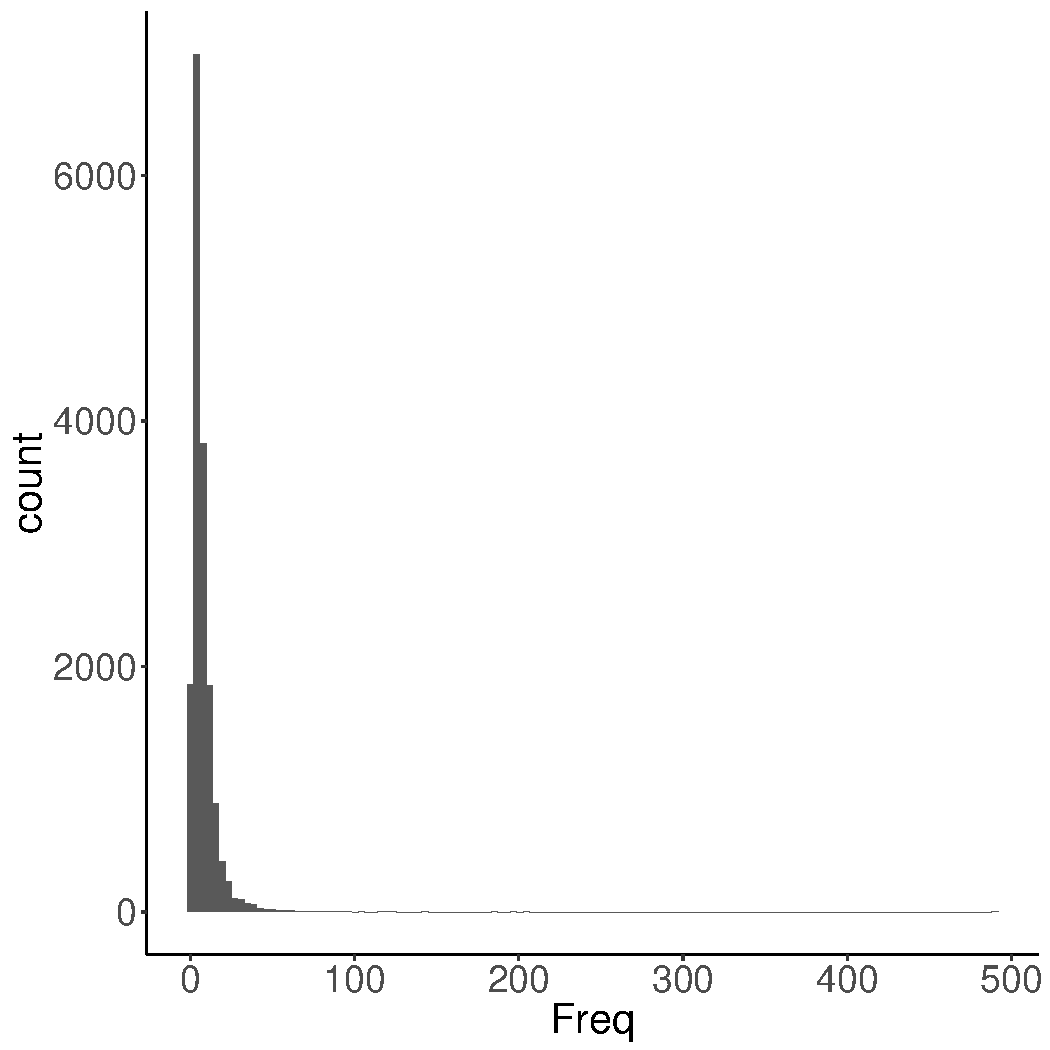
\includegraphics[width=0.6\linewidth]{figures/number_var_genes.pdf}
  \caption{Overall frequency of rare non-synonymous mutations.
    The range of rare variants per gene ranged from $3$ to $491$ with a median of $5$.
  }\label{fig:num_var}
\end{figure}

\subsubsection{Simulation Framework}
\label{ssub:Simulation_Framework}

From the set of $16,510$ genes I selected 50 genes at random which had at least 3 or more rare variants. 
Mutation were defined as rare if the minor allele frequency (MAF) was below or equal 1\%. 
Within $p$ rare variants of a gene I assigned causal status to $p_1 \ldots p_t$ positions, in which $t$ represents the total number of causal variants.
For simplicity I assigned the causal cluster at the beginning of the gene.
Within these simulations I gradually increased the size of the causal cluster to eventually cover the whole gene. 

The phenotype was simulated via a liability threshold model.
Hence the phenotype $Y_i$ of the $i^{th}$ subject was generated via
$Y = G\times E' + \epsilon$
in which $G$ is the standardized genotype matrix of $n=1000$ subjects with $p$ variants.
$E$ is the effect size vector of size $1\times p$ and $\epsilon$ is a standard normal distributed error term with a mean of $0$ and a standard deviation of $\sqrt{1-h^2}$, in which $h^2$ is the assumed heritability or the genetic effect on the liability distribution.
The effect $h$ was uniformly distributed across all causal variants.
I assigned case status for each subjects whose $Y_i$ is above a certain liability threshold $q$.
Any subject above $q$ was assigned case status, while the remaining subjects were deemed to be controls.
This process was repeated until $500$ cases and an equal number of controls were collected.

\subsubsection{Application of the KS-Burden}
\label{ssub:Application_of_the_KS-Burden}

The KS-Burden test was further applied to the UK BioBank to investigate distributional differences of rare variants between aggressive and non aggressive individuals.
As described in the previous chapter the UK BioBank is a chip-array data set.
Commonly genotyped data is not applicable for rare variant testing due to the low imputation quality of low frequency variants.
However, given a very large sample size, imputation quality is gradually improving thus allowing investigations of rare variants.
Indeed, the UK BioBank is with over $150,000$ samples relatively large.
Further, as can be seen in Figure~\ref{fig:imputation}, imputation quality is acceptable for variants with a frequency between 1\% and 0.1\%, given the commonly used quality score cut-off of $0.2$.
Therefore providing sufficient high quality variants to investigate potential distributional differences.

%\begin{figure}[htpb]
%  \centering
%  \includegraphics[width=0.8\linewidth]{example-image-a}
%  \caption{Imputation Quality of the UK BioBank}\label{fig:imputation}
%\end{figure}

\section{Results}
\label{sec:results}

\subsection{Genetic Correlation}
\label{sub:psych_genetic_correlation}

First, the genetic correlations between impulsive aggression and depressive symptoms is remarkably high ($r_g=0.6741$, $SE=0.0919$, $p=2.2326\times 10^{-13}$).
This high correlation is also reflected in subjects diagnosed with a major depression ($r_g=0.4134$, $SE=0.1212$, $p=6\times 10^{-04}$).
In contrast, correlations between impulsive aggression and Bipolar disorder was not significant after adjusting for multiple testing at $\alpha=0.00625$ ($r_g=0.1192$, $SE=0.0949$, $p=0.2091$).
Similar genetic correlations with Schizophrenia was not of large effect ($r_g=0.161$, $SE=0.0566$, $p=0.0045$) and failed to pass multiple testing.

In contrast correlations between risk taking and Bipolar ($r_g=0.2561$, $SE=0.0606$, $p=2.4034\times 10^{-05}$), as well as Schizophrenia ($r_g=0.232$, $SE=0.0431$, $p=7.3554\times 10^{-08}$) remained significant.
In addition, while genetic correlations were highly significant between aggression and depression, genetic correlations between risk raking, depressive symptoms ($r_g=0.0856$, $SE=0.0687$, $p=0.2129$) as well as MDD ($r_g=0.0028$, $SE=0.0853$, $p=0.974$) were small and did not pass the multiple testing threshold.

An overall overview of all genetic correlations are given in Figure~\ref{fig:ukb_psychiatric/figures/combined_corr.pdf}.

\begin{figure}[htpb]
  \centering
  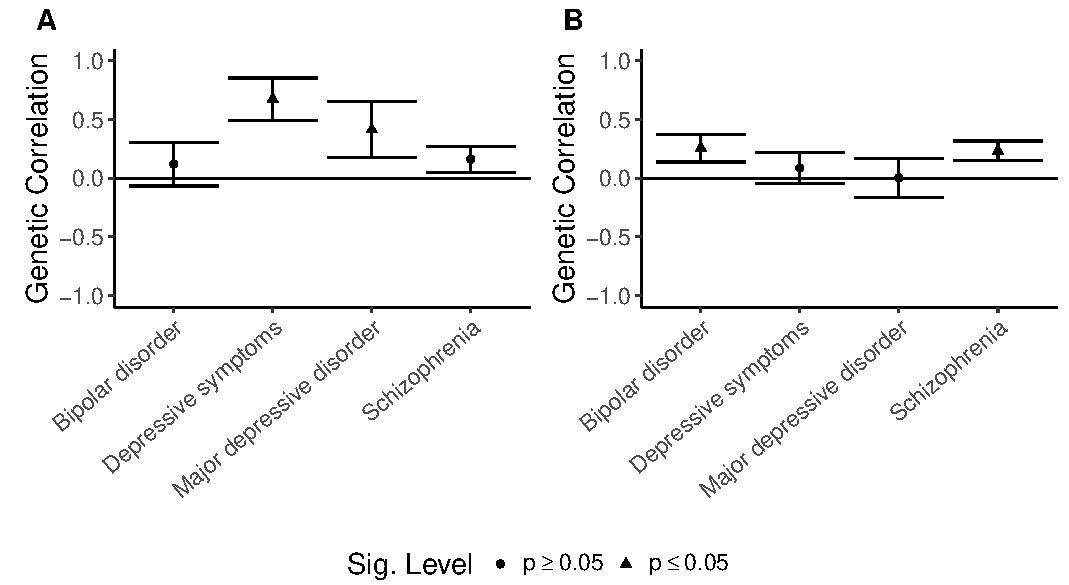
\includegraphics[width=0.8\linewidth]{ukb_psychiatric/figures/combined_corr.pdf}
  \caption{Genetic correlations between impulsive aggression and risk taking with selected psychiatric disorders.
    The error bars display the 95\% confidence intervals for each pairwise genetic correlations.
    Significance levels after multiple testing correction are displayed in form of a dot ($p\ge 0.05$) and triangle ($p\leq0.05$).
    (A) Genetic correlations between impulsive aggression and psychiatric disorders. 
    (B) Genetic correlations between risk taking and psychiatric disorders.
  }\label{fig:ukb_psychiatric/figures/combined_corr}
\end{figure}


\subsection{Mendelian Randomization}
\label{sub:mendelian_randomization}

Utilization of MR to infer potential causal influence of psychiatric disorders on aggression and risk taking yielded two potential links (Figure~\ref{fig:overall_mr_effect}).
While most methods agree with the direction of effect, MR-Egger commonly resulted in larger confidence intervals and did not resulted in any significant findings.
Nevertheless, MR-egger is known to be less powerful in cases where most used genetic variants are valid instruments.

MR analysis suggest some indication that SZ might causally influence both aggression and risk taking.
In particular, all applied methods, with the exception of MR-Egger, support the notion that SZ might both increase levels of risk taking as well as impulsive aggression.
In addition, there is little evidence for a possible MR assumption violation via pleiotropic effects.
Both funnel plots in Figure~\ref{fig:sensitivity} as well as MR-Egger intercepts (Figure~\ref{fig:sensitivity}) suggest little to no pleiotropy between instrument and outcome.
Further, these results seem not to be driven by outliers (see Figure~\ref{fig:mr_aggression} and Figure~\ref{fig:mr_risk}).
This indicates a potential causal effect of SZ on both risk taking and impulsive aggression.

Mixed results were obtained in the MR analysis investigating a potential causal effect of depression on aggressive behavior.
Depressive symptoms are suggested to cause an increase in impulsive aggression by all but MR-egger.
Specifically, MR-Egger regression indicates, while retaining an non-significant slope, the opposite direction of effect compared to other used methods.  
A possible explanation for this discrepancy can be found in potential pleiotropic effects which might violate MR assumptions (see Figure~\ref{fig:sensitivity}).
Indeed, inspection of the funnel plot in Figure~\ref{fig:sensitivity} shows considerable asymetry, thus suggesting the presents of pleiotropic effects.
In addition, the intercept of MR-egger regression differs significantly from $0$.
Thus, there is no evidence which could suggest a causal influence of depressive symptoms on aggression. 
Similar, but weaker, results were obtained from the MR analysis between MDD and impulsive aggression.
None, of the used methods suggested significant causal effects between the two phenotypes. 
Further, analysis of the funnel plot suggest a possible pleiotropy violation.

In addition, there is some indication of a causal effect of BP on risk taking.
However, these effects are rather weak across the used instruments.
Further, MR analysis was unable to identify causal effects of both DS and MDD on risk taking.
Also an effect of BP on impulsive aggression was not supported within this analysis.

\begin{figure}[htpb]
  \centering
  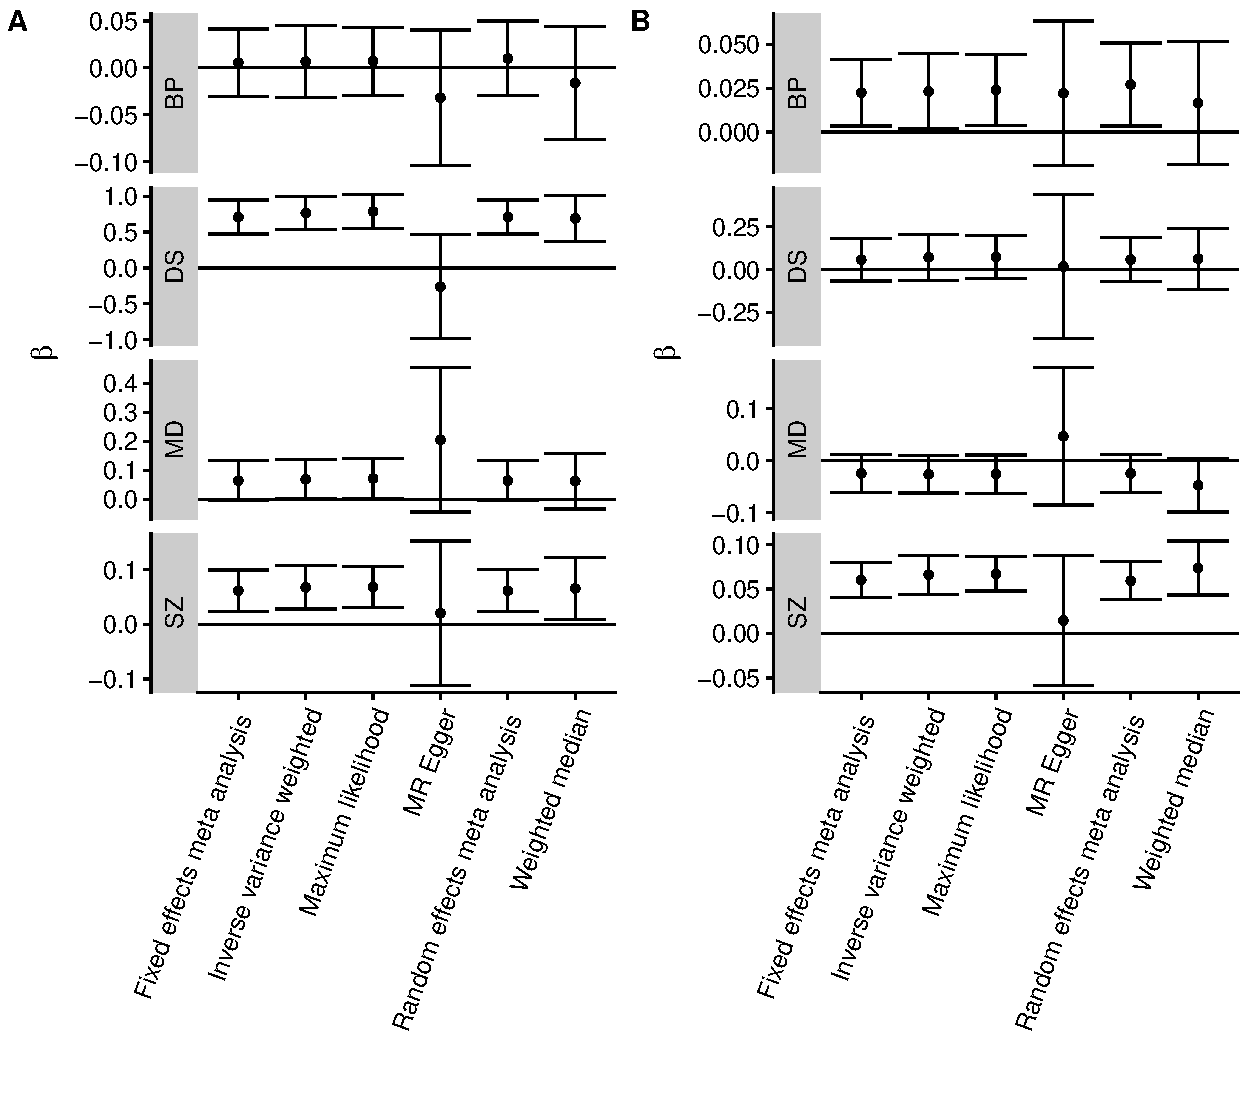
\includegraphics[width=0.9\linewidth]{ukb_psychiatric/figures/overall_mr_effect.pdf}
  \caption{Estimated causal effect of psychiatric disorders on impulsive aggression and risk taking.
    The effect size of the causal effect $\beta$ is displayed on the y-axis, while used Mendelian randomization methods are on the x-axis.
    SZ, Schizophrenia; MDD, Major Depressive Disorder; DS, Depressive Symptom's; BP, Bipolar Disorder.
    (A) Effect of psychiatric disorders on impulsive aggression.
    (A) Effect of psychiatric disorders on risk taking.
  }\label{fig:overall_mr_effect}
\end{figure}

\begin{figure}[htpb]
  \centering
  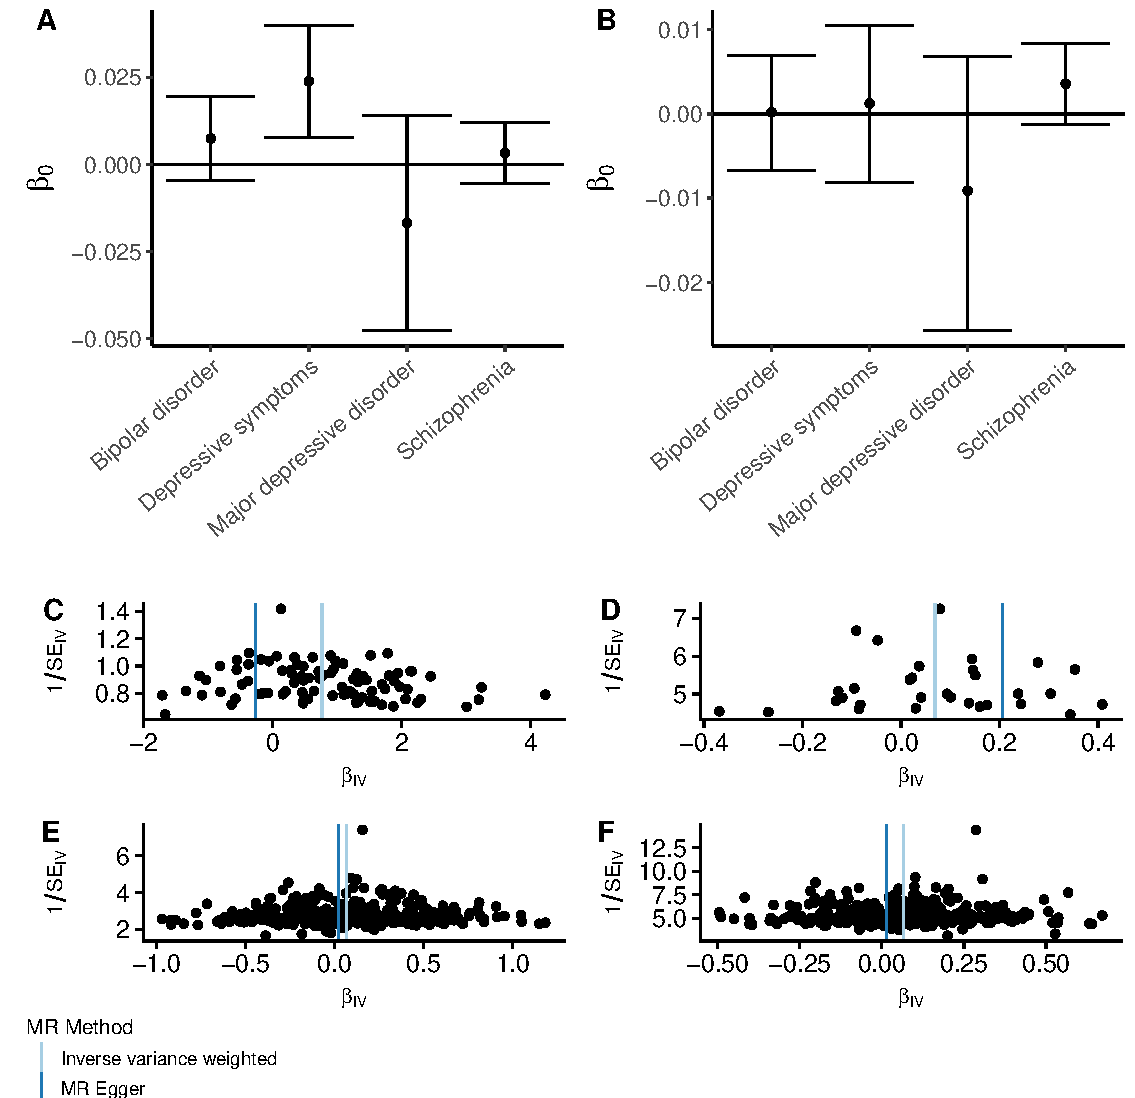
\includegraphics[width=0.9\linewidth]{ukb_psychiatric/figures/sensitvity_plot.pdf}
  \caption{Sensitivity analysis.
    (A) Displays the intercept $\beta_0$ of MR-egger regression for psychiatric disorders on impulsive aggression. The intercept is an indication of whether directional horizontal pleiotropy is driving the MR analysis.
    (B) The MR-egger regression intercept of psychiatric disorders on risk taking.
    (C) Funnel plot of Depressive symptoms on impulsive aggression. 
    (D) Funnel plot of MDD on impulsive aggression. 
    (E) Funnel plot of SZ on impulsive aggression. 
    (F) Funnel plot of SZ on risk taking. 
    The intercept of both MR-egger and Inverse variance method are indicated with a vertical line.
    Error bars indicate the 95\% confidence intervals.
  }\label{fig:sensitivity}
\end{figure}

The hypothesised direction between exposure and outcome were tested with the help of the Steiger test~\cite{Steiger1980}.
In general the test examines if the variance explained by the used instrumental SNP in the outcome is less than those within the exposure. 
Careful inspection of these test results suggest that there were no violation of the hypothesised direction of causal effects across all tested connections.

To conclude, careful examination of the here presented MR analysis gives some indication of a causal connection between SZ on both risk taking and impulsive aggression.
However, potential causal effects of other psychiatric disorders on aggression or risk taking was not supported.

%! TEX root = /home/robert/Documents/projects/thesis/header.tex

In the previous chapters I have investigated the genetic architecture of aggressive behavior.
I outlined previous studies which examined genetic factors affecting aggression and described general methodological approaches in identifying those.

My first study explored the longitudinal heritability of childhood aggression.
I showed that genetic factors, which influence aggression, are rather stable over age and that quantitative sex differences are minor.
Following, I analysed specific molecular markers which might influence both impulsive aggression and risk taking behavior.
I identified two independent SNPs associated with risk taking, but failed to detect any genome-wide signal for impulsive aggression.
Next, I investigated the relationship of impulsive aggression and risk taking with various psychiatric disorders.
I showed  high genetic correlations between impulsive aggression and depression (MDD and DS).
In addition, application of a Mendelian randomization demonstrated that schizophrenia might causally affect both impulsive aggression and risk taking.
Within my last study I investigated the properties of the KS-Burden test.
This test is designed to explore distributional differences of rare variants between affected and unaffected individuals.
The test showed generally better performance than other rare variant tests when clusters of causal variants were present.
Application of the KS-Burden test to examine the impact of rare variants on aggressive behavior did not result in any genome-wide significant findings, however.

Within this chapter I will discuss my findings in general.
First I am going to contrast heritability estimates from  my twin study and GWAS\@.
Following, I will explore the results of the association studies as well as implications for future studies.
Finally, I will discuss genetic correlations in general, followed by an examination of Mendelian randomizations.

\section{Heritability of Aggression}
\label{sec:heritability_of_aggression}

The missing heritability problem is well-known in genetics.
Thus, it is not surprising to find that heritability estimates from the twin study and those computed on SNPs differ.
Specifically, I showed that heritability of aggressive behavior in children is stable across age and ranged from 50 to 80\%, while the heritability estimate from the conducted GWAS was 5\%. 

First of all it is important to note that these two heritability estimates are not directly comparable.
Specifically, twin estimations were done on children while SNP heritability was derived from mostly middle-aged adults.
However, previous heritability estimations in adult twins were similar estimates to those in children~\cite{Miles1997a}.

The observed differences could also have been caused by the differences in instruments as well as the definition of aggressive behavior.
While both  twin studies made use of a validated psychometric instrument to measure aggressive behavior in children, measurements in the UK Biobank were based on a single question with dichotomous answers choices.
Thus, measurements within the UK Biobank are of less precision and potentially include more noise.
Furthermore, aggressive behavior within the UK Biobank was defined as an impulsive act while the  instruments in the twin studies assumed a more general definition of aggression.
Hence, the  instruments show a considerable degree of diversity in both definition and psychometric properties, potentially affecting heritability estimations.

The GWAS by~\citet{Pappa2016a} also demonstrated great variability across assessed cohorts in terms of SNP heritability of aggressive behavior in children as well ($10-54\%$).
However, it is unclear if these differences are due to genotyping platform, the age of included participants or assessment instrument.
Furthermore, 95\% confidence intervals across cohort estimates are overlapping indicating that differences in heritability are not statistically significant.
Indeed, only the two smaller cohorts of this particular study show relatively high heritability estimates ($h^2=.54, N=2,101; h^2=.46, N=908$), while the largest cohort displayed a similar estimate as the one presented in Chapter~\ref{cha:assocation_study_in_agggressive_behavior_and_risk_taking} ($h^2=.1, N=5,505$).
This suggests that estimated SNP heritability of impulsive aggression within the UK Biobank is similar to that estimated from validated psychometric instruments. 

However, there are a number of potential additional reasons for the observed discrepancy between twin and GWAS heritability estimates as I already described in Section~\ref{sec:heritability_and_genetic_correlation}.
GWAS rarely capture potential epistatic effects, discount the influence of rare variants, and are unable to investigate the influence of regulatory components. 
However, to what extent these additional factors influence the size of the observed discrepancy remains unknown.

Interestingly a study investigating family-based heritability estimations (i.e. using parent-offspring and sibling correlations) showed that models which did take shared environmental factors into account (using SEM), compared to those which did not (Falconer's method), resulted in heritability estimates closer to those seen in genotype data~\citet{Munoz2016a}.
However, this study only looked at diseases such as cardiovascular diseases, various forms of cancers, and diabetes.
Noticeable, the only behavioral  disorder assessed within this study, namely depression, showed the largest missing heritability.
A slightly different suggestion was made by~\citet{Yang2015} who argued that the missing heritability can be explained by taking rare variants into account.
Indeed, in their study rare and common variants were able to explain most of the missing heritability in BMI and height.
While it is unclear to which extent this seems also the case for other phenotypes, most studies to date failed to identify rare variants which were able to account for a considerable proportion of phenotyical variability in a complex trait~\cite{Chabris2015,Wray2011}.
Thus, one can speculate that the simplified instrument used with the GWAS, as well as the different operationalization, as well as definition of aggression has considerable contribution to the discrepancy, but other sources might also be possible.

However, the missing heritability should not distract from other interesting questions such as \acrfull{gxe}.
As shown in Section~\ref{sec:evolutionary_theories}, aggressive behavior has a variety of beneficial and harmful consequences, depending on environmental circumstances. 
For example, while aggressive behavior in social situations can be beneficial to gain social status, it can also be highly penalized by others in the group~\cite{Buss1997}.
Another example is the findings by~\citet{Figueredo1995} which showed that aggressive behavior of husbands towards their wives was profoundly affected by the distance or presence of brothers or powerful fathers.
These findings would suggest considerable environmental influence on the expression of aggressive behavior as well as possible gene-environment interactions (see \textit{MAOA}-environment interactions in Section~\ref{sub:maoa_interactions}).
However, these interactions will not appear in heritability estimates, or the ratio of genetic to total variance in a population.
%, which can also be described as the ratio of genetic and total variance in a population which shares a common environment.
Indeed, the presents of a hidden underlying environmental structure which interacts with genetic factors would push the genetic variance to the denominator.
Thus, reducing the heritability estimation.
Nevertheless, GxE effects might be able to explain a proportion of the total phenotypic variance.

To conclude, the study presented in Chapter~\ref{cha:assocation_study_in_agggressive_behavior_and_risk_taking} represents the first extensive investigation of the genetic architecture of adult human aggression.
The use of over $17,000$ twin pairs not only enabled a robust examination of genetic and environmental factors involved in childhood aggression, but also empowered a detailed analysis of potential sex and age differences (see Chapter~\ref{cha:longHera}).
This analysis demonstrated that sex and age only had a minor effect the estimated heritability.
I further showed that SNP heritability in impulsive aggression is  only 5\%, relatively small.
Next I will discuss my genetic association studies on impulsive aggressive behavior as well as risk taking. 

\section{Genomic Associations in Aggression and Risk Taking}
\label{sec:genomic_associations_in_aggression_and_risk_taking}

\subsection{Common Variants}
\label{sub:common_variants_discussion}

Within Chapter~\ref{cha:assocation_study_in_agggressive_behavior_and_risk_taking} I conducted a GWAS on both risk taking and impulsive aggression.
While I was able to replicate previous findings regarding risk taking~\cite{Day2016}, I was unable to identify any genome-wide signal for impulsive aggression.

Interestingly, genetic variants within \textit{CADM2} which were shown to influence risk taking are also associated with a number of other personality traits~\cite{Boutwell2017},
thus suggesting genetic overlap between risk taking and other personality characteristics.
Indeed, conditional FDR analysis (see Section~\ref{sub:conditional_fdr}) as well as genetic correlations (see Section~\ref{sub:genetic_correlation_ukb_assoc}) between risk taking and neuroticism suggest some overlap.

Furthermore, genetic variants associated with risk taking seem to be in close genomic proximity to those known to influence a proxy phenotype of smoking, namely spirometric measurements (the amount and speed of air a person can inhale/exhale).
Indeed, it is not clear to what extent as well as how risk taking and smoking behaviors are linked.
Previous research has shown that sensation seeking~\cite{Carton1994} and impulsivity~\cite{Glicksohn2007,Mitchell1999} is more prominent in smokers than non-smokers.
Furthermore, a study by~\citet{Ert2013} explored how smokers and non-smokers differ regarding risk taking and found that smokers are more easily tempted by high rewards,
thus suggesting that higher prevalence of risk taking behavior in smokers reflects an impulsive behavior to give into immediate temptations. 
One can therefore speculate that both traits might have shared genetic factors which influence both risk taking and smoking.
Indeed, genetic correlation analysis showed considerable genetic correlation between the two traits (see Chapter~\ref{cha:assocation_study_in_agggressive_behavior_and_risk_taking}).
However, an alternative explanation is that risk taking is causally influencing smoking status,
suggesting that an intervention which is aimed to reduce risk taking behavior might reduce smoking prevalence. 
Nevertheless, it is unclear how such a general personality trait can be experimentally modified to have a long-term health effect.

In contrast to risk taking I was unable to identify any genome-wide associations for impulsive aggression, despite estimating the heritability of aggressive behavior between 50--80\% (see Chapter~\ref{cha:longHera}).
A likely reason for the current failure to identify genome-wide significant variants is that the study presented in Chapter~\ref{cha:assocation_study_in_agggressive_behavior_and_risk_taking} as well as the similar study by~\citet{Pappa2016a} have limited statistical power.
While the study by~\cite{Pappa2016a} on aggression in young children and teenagers is limited to a relatively small sample size ($N=18,988$),
my study, with nearly twice as many subjects, measured aggressive behavior without the help of a validated psychometric instruments and consisted only of one single `yes' or `no' question, unlike~\citet{Pappa2016a}, which made use of well-known instruments to assess aggressive behavior.

Thus, it is obvious that an increase in sample size is necessary in order to boost statistical power.
However, it remains difficult to both obtain high quality phenotype data while increasing sample size to tens of thousands of participants.
The data obtained by~\citet{Pappa2016a}, as well as those used in Chapter~\ref{cha:longHera}, are based on multi-question instruments, commonly used with multiple raters.
While the validity of these tools has been shown multiple times~\cite{Goodman1997,Goodman2001,Achenbach2003}, it is difficult to see how these can be translated to studies with larger sample sizes.
This opens the need to develop instruments which can accurately measure aggressive behavior in a larger samples or validate pre-existing ones.  
For example, the  instrument to measure impulsive aggression in Chapter~\ref{cha:assocation_study_in_agggressive_behavior_and_risk_taking} has not been validated but could easily be explored in the context of other instruments such as CBCL and SDQ\@.
In addition, it is important to note that the distribution of aggression scores of both CBCL and SDQ (see Figure~\ref{fig:hist_aggression}) is skewed.
Therefore, a dichotomous instrument might be able to accurately assess aggressive behavior in larger samples. 

\subsection{Rare Variants}
\label{sub:rare_variants_disccusion}

Rare variants, in respect to impulsive aggression, were analysed in Chapter~\ref{cha:distribuional_differences_of_rare_variants}.
Specifically, I developed a new rare variant association test, called KS-Burden, in order to detect clusters of causal mutations within genomic regions such as genes.
While simulations have shown relatively good performance of KS-Burden compared to other tests, application to impulsive aggression yielded no genome-wide significant findings. 

There are multiple possible reasons for these null findings (see Section~\ref{sec:discussion_ks}).
Most notably, it remains unlikely that rare variants will have a considerable effect on behavioral traits.
Indeed, there is currently no study demonstrating considerable contribution of rare variants in explaining variation in behavioral phenotypes~\cite{Chabris2015}.
However, one could argue that these lack of findings are due to the small sample sizes commonly seen in sequencing-based studies~\cite{Lee2014}. 
In this respect, it is important to emphasis that, in contrast to the association study of common variants, the outlined rare variant association study has considerable statistical power~\cite{Lee2011}.
Specifically, while most studies which aim to explore the impact of rare variants only use a few hundred samples the study presented in Chapter~\ref{cha:distribuional_differences_of_rare_variants} was able to make use of over $30,000$ subjects. 
Thus, this well-powered study could suggest that the observed  null findings imply that rare variants are unlikely to have a major influence on impulsive aggression.

However, it is important to mention that the rare variant association study in Chapter~\ref{cha:distribuional_differences_of_rare_variants} made use of chip array data, a method which is unable to detect private mutations due to the limited number of SNPs adequately tagged.
Indeed, the~\acrfull{exac} has shown in a sample of $60,706$ unrelated individuals that the majority of rare mutations are private mutations (also called singletons), and that a large proportion of these mutations have potential disease implications~\cite{Lek2016,Kobayashi2017}.
However, this does not necessary imply that rare mutations might play an important role in common traits, such as aggression~\cite{Chabris2015}.
Nevertheless, rare, as well as private, mutations could be helpful in explaining extreme expressions of aggressive behavior.
For example, a study by~\cite{Peloso2016} recently showed that extreme phenotype selection results in a greater increase in statistical power in rare variants compared to common variants,
thus suggesting that future studies might look at highly violent criminal offenders in order to identify genes with higher burden of rare variants.

\section{Phenotypic and Genomic Correlations}
\label{sec:phenotypical_and_genomic_correlations}

As described in Chapter~\ref{cha:introduction}, the genetic overlap between aggression and other behavioral phenotypes was unknown.
Chapter~\ref{cha:assocation_study_in_agggressive_behavior_and_risk_taking} as well as Chapter~\ref{cha:psychiatric_corr_mr} explored these genetic relationships.
In particular, I have shown considerable genetic correlations between aggression and risk taking, as well as with neuroticism, smoking, and depression. 
Especially interesting is the unusually high genetic correlation between aggression and depression.

However, as described in Section~\ref{sec:heritability_and_genetic_correlation}, genetic correlations can arise from a multitude of different scenarios.
Thus, it remains unclear if these correlations arise from direct pleiotropic effects, are mediated by other variables, or are caused by other scenarios (see Figure~\ref{fig:genetic_correlation}). 
Indeed, while genetic correlations are able to give some insight into the biological interconnectedness of traits, they suffer some same problems as other correlational analysis. 
For example, the high genetic correlations between depression and aggression could be caused by underlying but unobserved third, fourth, or numerous other phenotypes.

In the past, genetic correlations were only measurable in twin and other genetically-informative studies, or with  raw genotype and phenotype data.
However, with the recent development of LD-score regression, researchers are now able to compute genetic correlations for     a number of phenotypes based on summary statistics alone.
While this had led to an explosion of genetic correlations~\cite{Bulik-Sullivan2015b,Bulik-Sullivan2015a}, it remains unclear how to interpret these genetic correlations regarding disease etiology.

There have been some efforts to understand genetic correlations in a more local sense.
\citet{Shi2016a} (under revision) showed that it is possible to partition genetic correlations across different genetic loci.
The authors showed that the cross trait correlations of 27 traits were mostly driven by only 27 genomic regions, and a number of small genome-wide genetic correlations were highly locally correlated.
While these attempts are important in order to foster our understanding of the shared biological mechanisms across different disorders, they also can be useful in order to understand potential causal relationships across traits.
Indeed,~\citet{Shi2016a} attempted to investigate putative causality by making use of genome-wide significant SNPs within correlation clusters.
For example, the authors demonstrated that the genome-wide correlation between \acrfull{bmi} and \acrfull{tg} can be explained by considering the local correlations around SNPs which were significant in BMI but not TG\@.
In contrast, the local genetic correlation of SNPs significant in TG  but not BMI was not significantly different from $0$.
Hence, suggesting that BMI might have a causal effect on TG\@.
However, while this method is an interesting approach it does not account for potential hidden variables.
Specifically, shared genetic variants might affect a related or sub-phenotype that might be pleiotropic for both BMI and TG\@.
Furthermore, more complex causal relationships, such as those often found in behavioral traits, might be less straightforward than the given example by~\citet{Shi2016a}.
Hence, while local genetic correlations might help to improve our biological understanding it does only partially improve the interpretation.

Another problem in the analysis of genetic correlations is that most summary statistics were obtained from different samples.
This is commonly seen as something positive, given that sample overlap can lead to a bias in the estimation of genetic correlations when using polygenic risk scores. 
However, LD score regression accounts for potential sample overlap~\cite{Bulik-Sullivan2015a} and gives an unbiased correlation estimate.  
Nevertheless, the availability of all relevant phenotype data within a single sample allows one to adjust for potential confounders already at the GWAS state.
This makes the UK Biobank especially useful and further methodological development might be directed at using classical regression methods to further elucidate causal interrelationships among phenotypes variables.

An additional interesting approach to further investigate genetic correlation structures is the use of Mendelian randomization.
I have used this popular approach in Chapter~\ref{cha:psychiatric_corr_mr} to demonstrated suggestive causal effects of schizophrenia on both risk taking and aggression.
However, there are a number of theoretical and practical issues which might lead one to question the validity of MR\@.

\subsection{Mendelian Randomization}
\label{sub:mendelian_randomization_discussion}

\subsubsection{Mendelian Randomization and Randomized Control Trials}
\label{ssub:causality_and_mendelian_randomization}

MR can be seen as similar to classical randomized control trials in which random genetic segregation  assigns subjects to either treatment or control group~\cite{Hingorani2005}.
However, as~\citet{Burgess2016a} pointed out, the aims of randomized control trials and MR are different.
While randomized control trials aim to evaluate the effectiveness of different treatment strategies, the main goal of MR is to assess the magnitude of the causal relationship between an exposure and an outcome. 
Only at a later stage MR aims to use this information to design non-genetic interventions.

This further implies that the effect of any designed intervention will differ from the genetically determined effects estimated by MR\@.
This is due to the length of the intervention (life long versus short term), the mechanism of intervention, as well as the magnitude of the intervention (genetic effects are usually small)~\cite{Evans2015}. 
Hence,~\citet{Vanderweele2015} questioned the use of  numerical estimates in MR and instead suggested testing only for the presences of a causal effect.

Thus, the results presented in Chapter~\ref{cha:psychiatric_corr_mr} have to be viewed in the context of experimental studies as well.
Indeed, as described in Section~\ref{sec:discussion_ukb_psych}, a number of randomized control trials support the notion of a causal relationship between schizophrenia and impulsive aggression as well as risk taking. 
However, it is unclear if other variables might mediate this relationship.

To conclude, while MR has been described in terms of randomized control trials there are some important differences.
However, MR can be useful in mining potential causal connections for future clinical trials~\cite{Evans2015}. 
In this regard it is important to emphasize that large-scale and hypothesis-free approaches to identify potential causal relationships in a large set of phenotypes need to be mindful regarding the underlying assumptions of MR\@.
Indeed, careful testing of assumptions might be difficult when exploring hundreds of potential causal connections,
thus increasing the chance of potential false findings.
However, MR can be a valuable tool in understanding the genetic correlations among multiple interconnected traits. 

\subsubsection{Instrument selection}
\label{ssub:instrument_selection}

A number of studies have been successful in identifying causal relationships between exposures and outcomes.
Most notable studies have shown causal effects of various traits, such has blood pressure, type-2 diabetes, and BMI, on cardiovascular disorders with the help of MR~\cite{Swerdlow,Ference2015,Lieb2013,Voight2012a}.
However, these successes were based on a biological understanding on how the instrument will affect the exposure in question.

This luxury is often not given in many other studies and information about the biological implications of associated variants is unknown.
This scenario is common in behavioral traits, psychiatric disorders, as well as other complex phenotypes.
Thus, some MR studies make use of statistically driven methods to chose SNPs as instrumental variables.
However, as~\citet{Burgess2016a} pointed out, studies which only use a statistically driven choice of instrumental variables and lack clear biological information are not true MR and might better be called `joint-association study' in which the underlying assumptions are only investigated post-hoc.

The lack of biological information has led to the development of new statistical methods to use multiple SNPs as instrumental variables. 
Indeed,~\citet{Burgess2016a} suggested that a specific causal effect of a risk factor on an outcome becomes more plausible if multiple SNPs, which are associated with the risk factor, agree with the effect.
For example,~\citet{Burgess2013} proposed to use allele scores as instrumental variables.
An allele score is either the weighted or unweighted sum of risk-increasing alleles for a given subject.
Indeed, usage of allelic scores from known biological markers facilitated correctly replicating known causal relationships~\cite{Timpson2005,CReactiveProteinCoronaryHeartDiseaseGeneticsCollaborationCCGC2011}.
However, while allelic score variants with known biological implications have been found to explain a considerable proportion of variance in specific traits, genome-wide scores demonstrated low specificity~\cite{Evans2013},
thus suggesting that there is currently little evidence which would recommend the use of genome-wide allelic scores as instruments.
Furthermore, allelic scores make use of raw genotype data thus limiting this approach to only a few locally available phenotypes.

In contrast, two-sample and meta-analysis approaches (see Chapter~\ref{cha:psychiatric_corr_mr}) can make use of summary statistics only to infer potential causal relationships. 
Since the effects of individual genetic variants are small, these methods commonly make use of multiple independent loci.
Here it is important to note that a strong effect size of a given SNP, used as instrumental variable, on the exposure does not suggest a strong causal connection between exposure and outcome, but rather represents the strength of the instrument.
A weak association between SNP and exposure, however, can result in an underpowered MR\@.

Similarly, it is unreasonable to assume that all genetic variants will fulfill all underlying assumptions.
Thus, multiple different methods have been developed in order to perform MR in the absence of clear biological information as well as to deal with possible assumption violations.

\subsubsection{Joint-Association studies}
\label{ssub:sensitivity_analysis}

\citet{Burgess2016a} suggested three different approaches to select genetic variants as potential instrumental  variables in the absence of biological knowledge.
(1) SNPs with indirect, but not conclusive, biological evidence.
These SNPs can be genome-wide associated genetic variants which have been replicated in multiple different populations.
(2) A more liberal approach would be to select genetic variants which are merely associated within a single population or sample.
This more liberal selection criteria is commonly used in the absence of clear biological information.
Sensitivity analysis can be used to investigate potential assumption violations, as done in Chapter~\ref{cha:psychiatric_corr_mr}.
(3) The most liberal approach is to use all available SNPs within the whole genome.
However, while this approach removes the necessity to justify  selection criteria of instrumental variables, it lacks theoretical legitimacy~\cite{Burgess2016a} and can result in a number of false findings~\cite{Evans2013}.

In Chapter~\ref{cha:psychiatric_corr_mr}, I made use of a liberal approach due to the lack of clear biological functional information.
On the basis of three GWAS on depression, schizophrenia, and bipolar disorder, I investigated potential causal effects on both risk taking and aggression.
Importantly, I chose a liberal $p$-value threshold for the inclusion of SNPs as instrumental variables.
A sensitivity analysis was used to investigate these findings for their robustness and, as shown in Figure~\ref{fig:sensitivity}, can provide valuable insight into possible assumption violations.

For example, funnel plots are commonly used to investigate potential directional pleiotropic effects.
Any asymmetry can be interpreted as a sign of directional pleiotropic effects.
However, the visual inspection of funnel plots can be questionable.
A few SNPs as instrumental variables can make the interpretation as either symmetric or asymmetric a difficult endeavour. 
This issue can also be seen in the funnel plots of Figure~\ref{fig:sensitivity}.
Specifically, the number of SNPs selected as instrumental variables for depressive symptoms and MDD are limited. 
Interestingly, one of the strongest assumptions of funnel plots, which are commonly used in a meta-analysis setting, might not be a problem in MR sensitivity analysis.

Within a traditional meta-analysis, funnel plots can provide an indication for potential publication bias.
However, they assume that effect size and sample size of each included study are uncorrelated~\cite{Evans2013}.
This is often not the case in many meta-analyses.
Indeed, studies might use different instruments to measure specific traits in small versus large samples or  might adjust sample size based on observed effect sizes of previous studies~\cite{Simonsohn}.
In contrast, the sample sizes of SNPs are rather constant.
Thus, funnel plots in MR do not suffer from the same problem.
Furthermore, in addition to funnel plots, potential pleiotropic effects can also be inspected by MR-egger's intercept (see Section~\ref{ssub:Used_Methods}).

An alternative explanation for an asymmetric funnel plot is that weaker instruments are more likely to be subject to the winner's curse~\cite{Taylor2014}.
The winner's curse was first described in the action theory literature~\cite{Bazerman1983} and states that the winning bid is likely to overestimate the true value of an item since it is the highest bid in the auction.
Similar in genome-wide association studies the focus is put commonly only  on significant SNPs, resulting in upwardly-biased effect size estimates.
This can lead to underpowered replication studies since sample size calculations are based on biased estimates~\cite{Xiao2008}.
Thus, instrument selection based on $p$-value alone can lead to an overestimation of the effect size between instrument and exposure, as well as  the association with the outcome~\cite{Bowden2015,Taylor2014}.
\citet{Burgess2016c} showed that this can lead to a bias in MR estimates when overlapping samples were used to estimate genetic association with the outcome and exposure.
Indeed, overlapping samples were present when MR analysis was performed between depressive symptoms and impulsive aggression as well as risk taking,
thus potentially explaining the asymmetry in the funnel plots at Chapter~\ref{cha:psychiatric_corr_mr}.

Furthermore, these careful post-hoc analyses can be seen as too weak in contrast to the strong assumptions made my MR\@. 
Thus, \citet{Vanderweele2015} suggested that negative results might be more plausible when investigating potential causal connections.
In particular, in light of the strong assumptions as well as inability to fully verify those assumptions, empirically it might be more beneficial to test assumed causal relationships with the help of MR\@.
However, this would require well-powered studies with large sample sizes.
Indeed, the UK Biobank as well as recent other consortia have shown that it is possible to acquire large samples.
While null results are not immune to biases, such bias would need to align perfectly in order to achieve an effect size of zero with a narrow confidence interval when in fact a true effect is present.
An obvious drawback from this approach would be its inability to discover new interventions for various disorders. 

Furthermore, it is important to emphasize that MR cannot make conclusive statements about the causal relationship between two variables.
In order to establish a causal relationship, a string of multiple evidence is necessary.
MR can only play a part in this and numerous other additional studies are necessary to confirm a causal relationship.
Furthermore, it is important to remember that in contrast to randomized control trials, MR commonly aims to detect small effect sizes.

To conclude, `joint-analysis' studies are able to identify potential causal relationships without clear biological insight.
While empirical methods exist to test the underlying assumptions, only additional evidence by randomized control trials or other forms of studies will be able to fully confirm any potential causal relationship.

\section{Conclusion}
\label{sec:conclusion}

Aggressive behavior is a heritable trait which shows strong genetic correlations with a number of other phenotypes, such as smoking and risk taking.
However, it remains unclear  how to interpret genetic correlations in general and what implications these estimates have in explaining the underlying architecture of aggressive behavior.
Mendelian randomization might be able to elucidate possible causal relationships among traits, but application of such methods needs to be done with care while respecting the underlying strong assumptions. 
Nevertheless, a careful application of such techniques has shown that schizophrenia might have a causal effect on both risk taking and impulsive aggression.

My current genome-wide association studies lack statistical power to detect specific genetic variants associated with aggression, yet is the largest ever conducted.
Future studies should aim to increase sample size as well as improve phenotyping quality.
Furthermore, while simulations have shown that the newly-developed methods are better able to detect clusters of rare variants, those clusters seem not to be present for impulsive aggression.

\end{document}

\subfile{ukb_assoc/ukb_assoc.tex}
\end{document}
